\documentclass{article}
\usepackage{amsmath}
\usepackage{graphicx}
\author{Chang Liu ~\\ chang\_liu@student.uml.edu}
\title{91.673 Advanced Database Systems Homework4}
\begin{document}

\maketitle

\section{Problem 1:Exercise 5.1.2}

\textbf{Exercise 5.1.2}: Compute the PageRank of each page in Fig. 5.7, assuming $\beta$ = 0.8. ~\\
\begin{center}
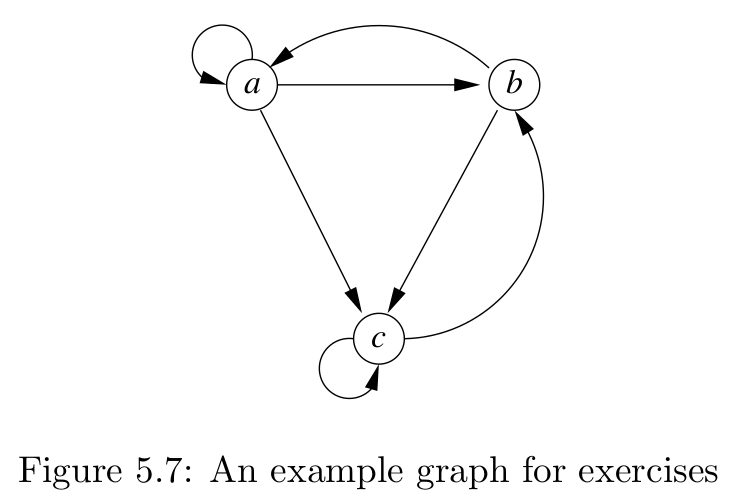
\includegraphics[scale=0.3]{hw3-figure5_7.png}
\end{center}


\section{Problem 2: Exercise 5.3.1}
\textbf{Exercise 5.3.1}: Compute the topic-sensitive PageRank for the graph of Fig.5.15, assuming the teleport set is:

(a) A only.

(b) A and C.



\section{Problem 3: Exercise 6.1.5}

\textbf{Exercise 6.1.5}: For the data of Exercise 6.1.1, what is the confidence of the
following association rules?

(a) $\{5, 7\} \rightarrow  2$.

(b) $\{2, 3, 4\} \rightarrow 5$.




\section{Problem 4: Exercise 6.2.6 (a)}

\textbf{Exercise 6.2.6}: Apply the A-Priori Algorithm with support threshold 5 to the data of:

(a) Exercise 6.1.1.



\section{Problem 5: Exercise 7.3.1}


\textbf{Exercise 7.3.1}: For the points of Fig. 7.8, if we select three starting points using the method
of Section 7.3.2, and the first point we choose is (3,4), which other points are selected.




\end{document}

